\documentclass[final,hyperref={pdfpagelabels=false}]{beamer}
\usepackage{grffile}
\mode<presentation>{\usetheme{I6pd2}}
\usepackage[english]{babel}
\usepackage[latin1]{inputenc}
\usepackage{amsmath,amsthm, amssymb, latexsym}
\usepackage{tikz}
\usetikzlibrary{shapes.geometric, arrows,backgrounds,fit}
\usepackage{booktabs}
\usepackage{caption}
\captionsetup{justification={justified}}
\usepackage[square,numbers]{natbib}
\usepackage{ragged2e}
\tikzstyle{arrow} = [thick,line width=0.8mm,->,>=stealth]
\usepackage{hyperref}

%\usepackage{times}\usefonttheme{professionalfonts}  % obsolete
%\usefonttheme[onlymath]{serif}
\boldmath
\usepackage[orientation=portrait,size=a0,scale=1.4,debug]{beamerposter}
% change list indention level
% \setdefaultleftmargin{3em}{}{}{}{}{}


%\usepackage{snapshot} % will write a .dep file with all dependencies, allows for easy bundling

\usepackage{array,booktabs,tabularx}
\newcolumntype{Z}{>{\centering\arraybackslash}X} % centered tabularx columns
\newcommand{\pphantom}{\textcolor{ta3aluminium}} % phantom introduces a vertical space in p formatted table columns??!!
\setbeamercolor{background canvas}{bg=lightgray}
\setbeamercolor*{block body}{bg=white, fg=black}
\listfiles
%%%%%%%%%%%%%%%%%%%%%%%%%%%%%%%%%%%%%%%%%%%%%%%%%%%%%%%%%%%%%%%%%%%%%%%%%%%%%%%%%%%%%%
\graphicspath{{figures/}}
 
\title{
\huge Collaborative Text Filtering \\
\Large The Mean Squares
}
\author{Peter J. Bakke (s183268), Daniel Horvath (s172185), Christian Hansen (s146498) and Thomas Brenner (s181857)}
\institute[Department]{\small DTU Compute, Technical University of Denmark}
\date[December. 17th, 2018]{December. 17th, 2018}

%%%%%%%%%%%%%%%%%%%%%%%%%%%%%%%%%%%%%%%%%%%%%%%%%%%%%%%%%%%%%%%%%%%%%%%%%%%%%%%%%%%%%%
\newlength{\columnheight}
\setlength{\columnheight}{105cm}

\begin{document}

\begin{frame}
 \begin{columns}
% ---------------------------------------------------------%
% Set up  COLUMN 1
% ---------------------------------------------------------%
 \begin{column}{.49\paperwidth}
 \begin{beamercolorbox}[center,wd=\textwidth]{postercolumn}
 \begin{minipage}[T]{.99\textwidth}  % tweaks the width, makes a new \textwidth
 \parbox[t][\columnheight]{\textwidth}{ % must be some better way to set the the height, width and textwidth simultaneously
                                                            % Since all columns are the same length, it is all nice and tidy.  You have to get the height empirically

% ---------------------------------------------------------%
% set up block  INTRODUCTION
% ---------------------------------------------------------%
\begin{block}{Introduction}
 \begin{columns}
 \begin{column}{1\textwidth}



\centering
\begin{minipage}[t]{0.98\textwidth}

\footnotesize{Collaborative text filtering is one of the most popular and effective approaches for recommender systems. Recommender systems are based on the idea, that given previously collected data about users and their interactions with items, you can predict whether a given user wants to have an interaction with a given item. This is widely used for platforms like Netflix, Amazon, Youtube and news websites. These platforms can increase their profits by being able to predict their consumers interests and showing content relevant for the user. 

The purpose of this project is to match two text descriptions of varied lengths. More concretely we propose a model to recommend articles to users based on the abstracts from other articles a user has indicated as read.
\vspace{0.5cm}
}



\end{minipage} \hspace{1cm}


      
\end{column}
 \end{columns}
 \end{block}
 \vfill


% ------------------------------------------------
% set up block METHODOLOGY
% ------------------------------------------------

\begin{block}{General Methodology}
 \begin{columns}
 \begin{column}{1\textwidth}


\centering
\begin{minipage}[t]{0.98\textwidth}

\footnotesize{
In general we try to maximize the probability of a match between a user and an item given some features: 
%
\begin{align*}
\max p (m | K; \theta)
\end{align*}
%
where $m$ denotes the binary variable on whether there is match, $K$ denotes the features, and $\theta$ denotes the parameters in the model.

To predict a users preferences we use
%
%
\begin{align*}
    p(m) = \sigma( f ( \text{UserId, MovieId}) ) 
\end{align*}
%
where $\sigma( \cdot )$ denotes the sigmoid function and $f( \cdot )$ is some function of users and items. In the matrix factorization $f(\cdot)$ could be given by the inner product of embeddings of users and items, e.g.:
%
%
\begin{align*}
    f(\cdot) = u \cdot m^T
\end{align*}
%
%
where
%
%
\begin{align*}
    u &= \text{Embedding}(x_u) \\
    m &= \text{Embedding}(x_m) 
\end{align*}
%
%
When we turn to the more advanced models $f(\cdot)$ is e.g. a neural net or LSTM net with user/item embeddings as input features instead of a simple inner product between the two, \cite{paragraph_embedding_comparison, Embedding, doc2vec}.
\vspace{0.5cm}
}



\end{minipage} \hspace{1cm}


      
\end{column}
 \end{columns}
 \end{block}
 \vfill

% ---------------------------------------------------------%
% set up block  DATA
% ---------------------------------------------------------%

 \begin{block}{Data}
 \begin{columns}
 \begin{column}{1\textwidth}
 


\vspace{-0.5cm}

\begin{minipage}[t]{0.98\textwidth}
\begin{itemize}
\justifying
\footnotesize{
        \item We use the publicly available \textbf{MovieLens} dataset from \url{https://grouplens.org/datasets/movielens/} for the first part of our project
	\item We use the publicly available \textbf{CiteULike} from \url{http://www.citeulike.org/faq/data.adp} for the second part of our project
}
\end{itemize}


\end{minipage} 



\vspace{0.5cm}

					
          
\end{column}
\end{columns}
\vskip-1ex
\end{block}
\vfill



% ---------------------------------------------------------%
% set up block  DATA
% ---------------------------------------------------------%

 \begin{block}{Key points}
 \begin{columns}
 \begin{column}{1\textwidth}
 


\vspace{-0.5cm}

\begin{minipage}[t]{0.98\textwidth}
\begin{itemize}
\justifying
\footnotesize{
        \item We construct a baseline model using \textbf{Matrix Factorization} on the MovieLens and CiteUlike datasets
	\item We construct a \textbf{Collaborative Text Filtering} model on the same data using
	{\setbeamertemplate{itemize items}[ball]
	\begin{itemize}
	\footnotesize{
	\item  \quad Feed Forward Networks, \cite{ncf2017, nielsenneural} 
	\item  \quad LSTM Networks, \cite{lstm1997}}
	\end{itemize}}
	And compare the results to the baseline model, \cite{lcmr2018, itemBasedCF2001, HU2008CollaborativeFF}
	\item We implement the models using the \textbf{Pytorch} deep learning framework and use \textbf{TorchText} for creating word embeddings and batch iterators
	\item We train the models using virtual machines on the \textbf{Google Colab} GPU cloud
}
\end{itemize}


\end{minipage} 
%\end{minipage} \hspace{1cm} \begin{minipage}[t]{.5\textwidth}


\vspace{0.5cm}

					
          
\end{column}
\end{columns}
\vskip-1ex
\end{block}
\vfill




% ---------------------------------------------------------%
% set up block  MovieLens
% ---------------------------------------------------------%


 \begin{block}{MovieLens}
 \begin{columns}
 \begin{column}{1\textwidth}


%\vspace{0.5cm}

\centering
\begin{minipage}[t]{0.96\textwidth}
			

\hspace{0.5cm} 
\vspace{-1cm}
\begin{columns}
 \begin{column}{0.60\textwidth}
 \justifying
 \footnotesize{
	The MoveieLens dataset consist of 20 million ratings on a scale from 0.5 to 5, of 27,000 different movies by 138,000 users. Taking outset in the MovieLens dataset the objective is to predict how a specific user will rate a specific movie. Figure \ref{fig:simple_cf_movielens} display the architecture we use in the simple collaborative filtering neural network for the MovieLens dataset.
	
		Table \ref{res:MovieLens_results} show the root mean squared error (RMSE) for the matrix factorization and the simple collaborative filtering neural network on the MovieLens dataset. For comparison we have included the RMSE from FastAI that use a similar model on the same dataset.
	
	The Figures \ref{fig:movielens_mf} and \ref{fig:movielens_nn} show how the matrix factorization and simple collaborative filtering neural network trains on the MovieLens dataset.
	
%	Figure \ref{fig:movielens_nn} show how the simple collaborative filtering neural network model trains on the MovieLens data set. The model is able to achieve around 40\% accuracy on the validation set. The result is not quite as good as we have hoped for, especially as it seems like the model is not learning a lot over the Epochs.
}
 \end{column}
 \begin{column}{0.39\textwidth}

\begin{table}[h]
\small
\centering
\caption{Results}
\label{res:MovieLens_results}
\begin{tabular}{lc}
\toprule
Model  & RMSE\\
\midrule
Matrix Factorization      &  0.895 \\
Neural Network - FastAI      &  0.889  \\
Neural Network - our result      &  0.881\\
\bottomrule

\end{tabular}
\end{table}

 \end{column}
 \end{columns}
 
 \begin{figure}

\includegraphics[width=0.75\textwidth]{movielensnet.png}
 \caption{MovieLens neural net representation} \label{fig:simple_cf_movielens}
\end{figure}  

\begin{columns}
 \begin{column}{0.49\textwidth}
 %\justifying
 %\footnotesize{
	
%	Table \ref{res:MovieLens_results} show the root mean squared error (RMSE) for the matrix factorization and the simple collaborative filtering neural network on the MovieLens dataset. For comparison we have included the RMSE from FastAI that use a similar model on the same dataset.
	
%	Figure \ref{fig:movielens_nn} show how the simple collaborative filtering neural network model trains on the MovieLens data set. The model is able to achieve around 40\% accuracy on the validation set. The result is not quite as good as we have hoped for, especially as it seems like the model is not learning a lot over the Epochs.}
\begin{figure}

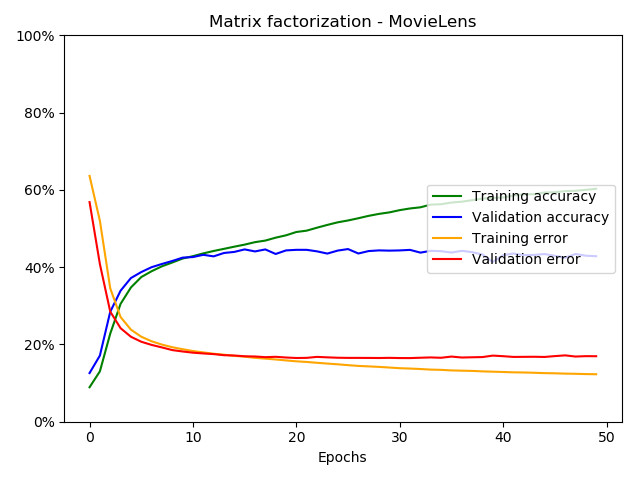
\includegraphics[width=0.75\textwidth]{MatrixFactorization_MovieLens.jpg}
 \caption{Training and Validation loss and Accuracy for the Matrix Factorization} \label{fig:movielens_mf}
\end{figure}  

 \end{column}
 \begin{column}{0.49\textwidth}

 \begin{figure}

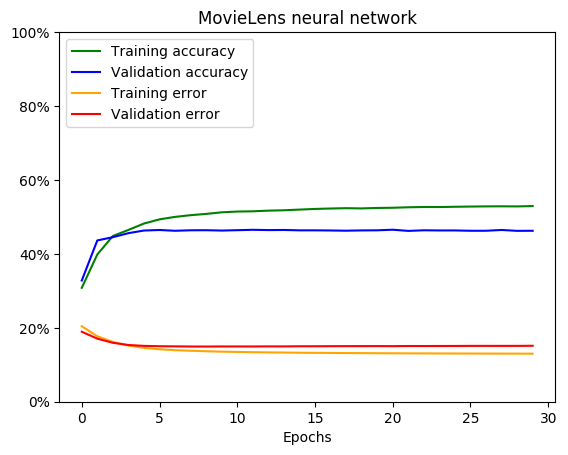
\includegraphics[width=0.75\textwidth]{movie_lens_res.png}
 \caption{Training and Validation loss and Accuracy for the Neural Network} \label{fig:movielens_nn}
\end{figure}  

 \end{column}
 \end{columns}




\end{minipage}



\vspace{0.5cm}

					
                  
\end{column}
\end{columns}
\vskip-1ex
\end{block}
\vfill






}
\end{minipage}
\end{beamercolorbox}
\end{column}
% ---------------------------------------------------------%
% end the COLUMN 1
% ---------------------------------------------------------%
 

% ---------------------------------------------------------%
% Set up COLUMN 2
% ---------------------------------------------------------%
    
\begin{column}{.49\paperwidth}
\begin{beamercolorbox}[center,wd=\textwidth]{postercolumn}
\begin{minipage}[T]{.99\textwidth} % tweaks the width, makes a new \textwidth
\parbox[t][\columnheight]{\textwidth}{ % must be some better way to set the the height, width and textwidth simultaneously
            											% Since all columns are the same length, it is all nice and tidy.  You have to get the height empirically
            

 \begin{block}{CiteULike}
 \begin{columns}
 \begin{column}{1\textwidth}


\centering
\begin{minipage}[t]{0.96\textwidth}
			

\hspace{0.5cm} 
\vspace{-1cm}
\begin{columns}
 \begin{column}{0.45\textwidth}
 \justifying
 \footnotesize{
	The CiteULike dataset consist of users represented by an Id and articles represented by an Id, the article Title and the article Abstract. The user-article interaction is represented as a binary attribute on whether a specific userId has put an ArticleId in his/her "basket". The modelling aim is to build a model that can recommend articles to users based on what they have previously read. }
 \end{column}
 \begin{column}{0.49\textwidth}

\begin{table}[h]
\small
\centering
\caption{Results} 
\label{res:CuL_results}
\begin{tabular}{lcc}
\toprule
Model  & Val. Accuracy        & \#Epoch         \\
\midrule
MF  	&  74\%        	 & 20           \\
FNN	  &  58\%        & 3         \\
LSTM	&  84\%        & 15         \\
\bottomrule
\end{tabular}
\end{table}

 \end{column}
 \end{columns}
 
 \begin{figure}

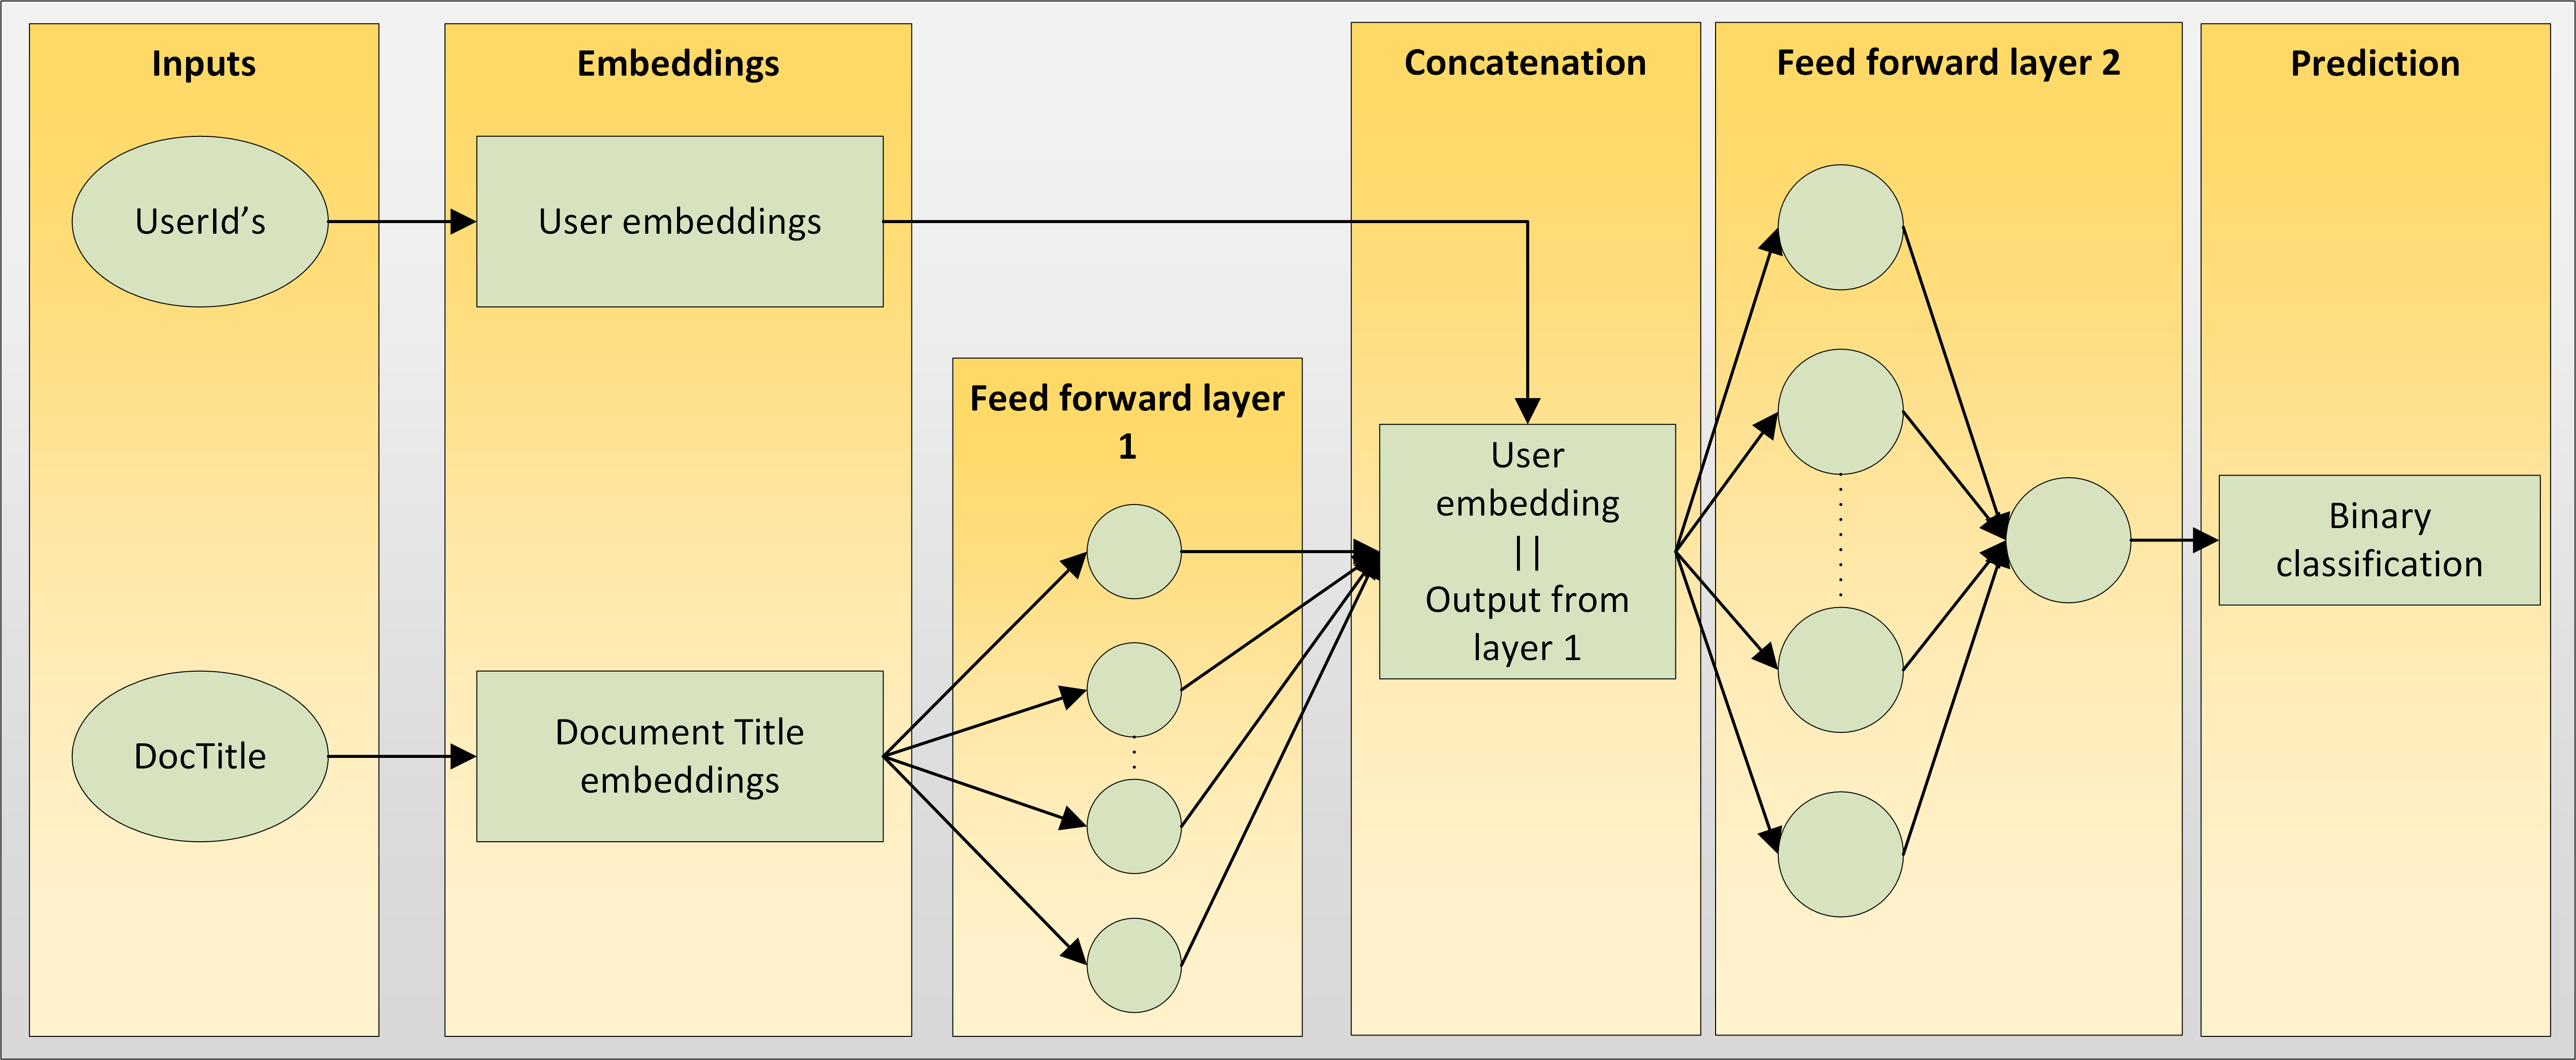
\includegraphics[width=0.95\textwidth]{CiteuLikeNet.png}
 \caption{CiteULike Neural net representation} \label{fig:CuL_net}
\end{figure}  

\begin{figure}

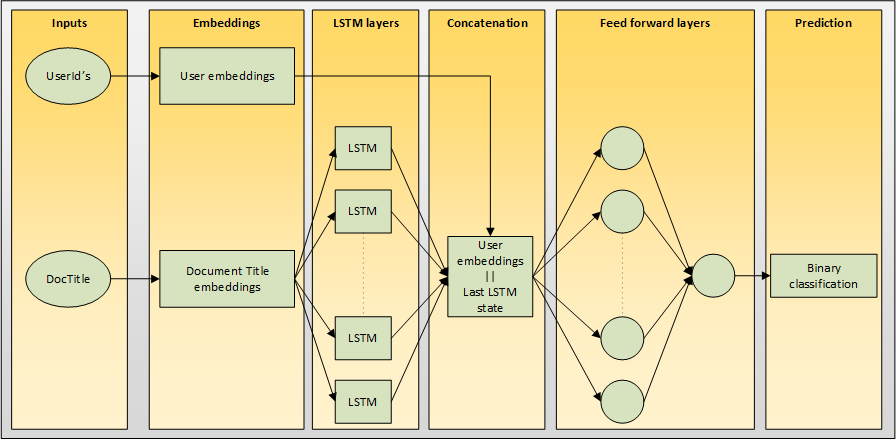
\includegraphics[width=0.95\textwidth]{CiteuLikeLSTM.png}
 \caption{CiteULike LSTM net representation. For clarity the temporal structure of the LSTM blocks have not been shown.} \label{fig:CuL_lstm_net}
\end{figure}


\begin{columns}
 \begin{column}{0.33\textwidth}
 

	\begin{figure}

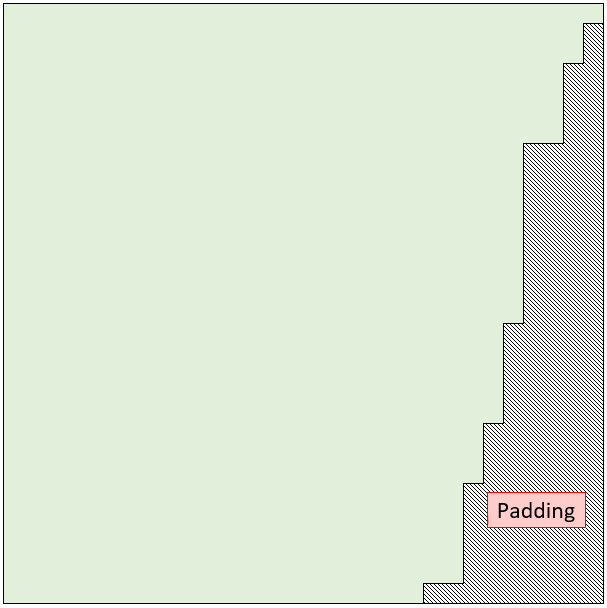
\includegraphics[width=0.75\textwidth]{sorted_batch.png}
 \caption{Batch sorting} \label{fig:batch_sorted}
\end{figure}

 \end{column}
 \begin{column}{0.66\textwidth}
	\justifying
 \footnotesize{
	Figure \ref{fig:CuL_net} show the simple collaborative filtering neural network architecture used on the CiteULike dataset. Figure \ref{fig:CuL_lstm_net} show the architecture of the collaborative filtering network enhanced with a number of LSTM layers and blocks.
	
	When training the model we need to take into account that the sequences are of varying length in order to not waste too much computation on calculating on the padding. Figure \ref{fig:batch_sorted} visualize how the amount of padding (the grey area) is minimized in the batch by sorting the documents on the length of the sentences.
	
	Table \ref{res:CuL_results} show the best achieved accuracy on the validation set in the three different models together with how many Epochs it took to reach that result.
	}
 \end{column}
 \end{columns}


\begin{columns}
 \begin{column}{0.49\textwidth}
% \justifying
% \footnotesize{
%	Figure \ref{fig:lstm_results} show how the LSTM model trains on the CiteULike data set. The model is able to achieve around 80\% accuracy on the validation set. The 80\% accuracy is a pretty good result since we right now only train on the Titles of the articles. We will try to improve the accuracy by training on the article Abstracts which contain a lot more information about the content of the article compared to the Title.}


\begin{figure}

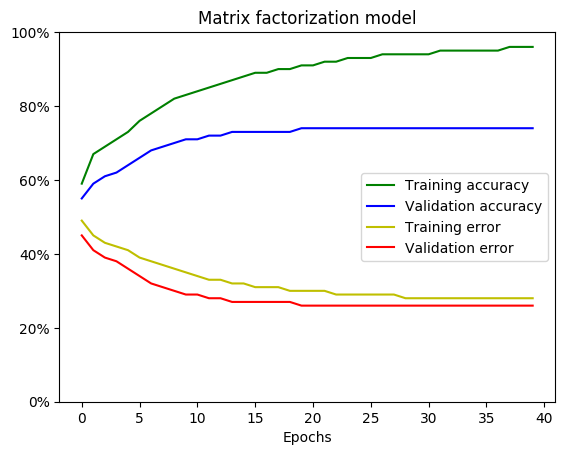
\includegraphics[width=0.75\textwidth]{matrix.png} 
 \caption{Training and Validation loss and Accuracy for the Matrix Factorization on the CiteULike data} \label{fig:CuL_mf}
\end{figure}

 \end{column}
 \begin{column}{0.49\textwidth}

\begin{figure}

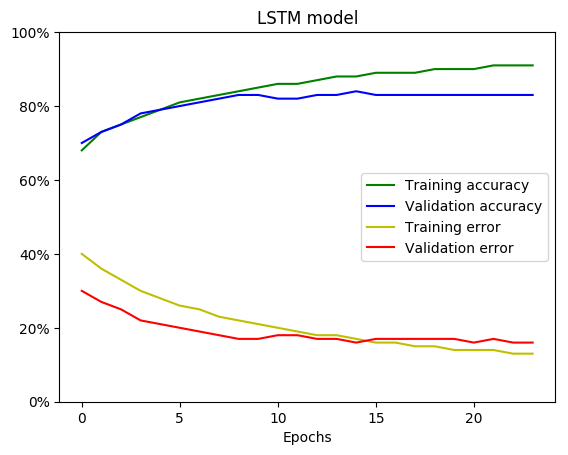
\includegraphics[width=0.75\textwidth]{lstm.png} 
 \caption{Training and Validation loss and Accuracy for the LSTM net on the CiteULike data} \label{fig:lstm_results}
\end{figure}

 \end{column}
 \end{columns}



\end{minipage}





\vspace{0.5cm}

					
                  
\end{column}
\end{columns}
\vskip-1ex
\end{block}
\vfill	

%\begin{block}{Comparison of results}
%
%\begin{columns}
%\begin{column}{1\textwidth}
%
%\centering
%
%%\vspace{2.5cm}
%\centering
%\begin{minipage}[t]{.95\textwidth}
%
%
%\vspace{-1cm}
%\begin{table}[h]
%\footnotesize
%\caption{Another table to summarize results - or maybe some more charts???}
%\begin{tabular}{p{8cm}p{2cm}p{2cm}p{2cm}p{2cm}p{2cm}p{2cm}p{2cm}p{2cm}p{2cm}p{2cm}p{2.5cm}p{2.5cm}}
%\toprule
%Location      & \multicolumn{10}{l}{What can we possibly show???}        & another metric & AUC or??? \\
%\midrule
%MovieLens MF          & 680 & 103 & 4   & 5   & 2   & 8   & 1   & 2  & 2 & 1 & 0.842 & 0.784 \\
%MovieLens NN         & 94  & 361 &  7  & 18  & 5   & 4   & 3   & 8  & 1 & 7 & 0.711 & 0.608 \\
%CuL MF    & 3   & 5   & 365 &  5  & 5   & 4   & 2   & 0  & 4 & 0 & 0.929 & 0.907 \\
%CuL NN     & 9   & 21  & 0   & 247 &  0  & 5   & 14  & 2  & 1 & 3 & 0.818 & 0.812 \\
%CuL LSTM     & 5   & 15  & 6   & 1   & 203 & 20  & 1   & 4  & 18& 0 & 0.744 & 0.732 \\
%\bottomrule
%
%\end{tabular}
%\end{table}
%
%
%\end{minipage}
%
%\end{column}
%\end{columns}
%\end{block}
%
%\vfill
\begin{block}{Acknowledgements}
\centering
\begin{minipage}[t]{0.98\textwidth}

\footnotesize{The authors wish to thank Alexander R. Johansen and Jose Juan Almagro Armenteros from DTU Lyngby for their constructive feedback and fruitful discussions during the process of the project.}
\end{minipage}
\end{block}
\vfill

\begin{block}{References}

{\scriptsize
\bibliographystyle{abbrvnat}	
\bibliography{biblio}
}			
\end{block}
\vfill


         
}
\end{minipage}
\end{beamercolorbox}
\end{column}
\end{columns}	
% ---------------------------------------------------------%
% end the COLUMN 2
% ---------------------------------------------------------%
  
  
\vskip1ex
%\tiny\hfill\textcolor{ta2gray}{Created with \LaTeX \texttt{beamerposter}  \url{http://www-i6.informatik.rwth-aachen.de/~dreuw/latexbeamerposter.php}}
\tiny\hfill{Created with \LaTeX \texttt{beamerposter}  \url{http://www-i6.informatik.rwth-aachen.de/~dreuw/latexbeamerposter.php} \hskip1em}
\end{frame}
\end{document}